154. \begin{figure}[ht!]
\center{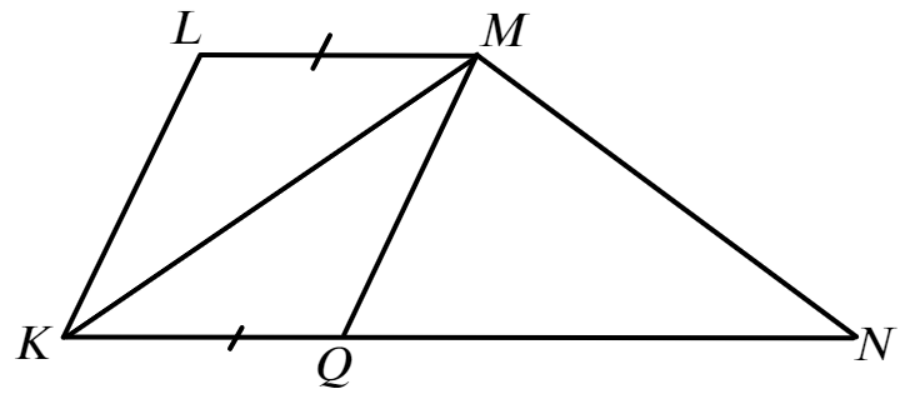
\includegraphics[scale=0.35]{g8-154.png}}
\end{figure}\\
Так как $(LM)\parallel (KQ)$ и $(MQ)\parallel(LK),$ четырёхугольник $KLMQ$ является параллелограммом, а значит $KQ=LM.$ Тогда $QN=KN-KQ=\cfrac{7}{4}KQ-KQ=\cfrac{3}{4}KQ,$ то есть $KQ:NQ=4:3.$ У треугольников $KMQ$ и $QMN$ общая высота из точки $M,$ значит $\cfrac{S_{\Delta KMQ}}{S_{\Delta QMN}}=\cfrac{KQ}{NQ}=\cfrac{4}{3}$ и $S_{\Delta KMQ}=\cfrac{4}{3}\cdot21=28.$ Диагональ $KM$ делит параллелограмм $KLMQ$ на два равных треугольника, значит $S_{\Delta KLM}=S_{\Delta KMQ}=28.$ Таким образом, $S_{KLMN}=21+28+28=77.$\\
